% =============================================================================
% Informe Tarea 1 — CMS y CountSketch en ventanas deslizantes.
% Formato de estilo tomado de S2/EDAA/tools/formatoInforme/formatoInforme.tex.
% Compilar con pdfLaTeX (Overleaf): subir esta carpeta completa (informe.tex,
% escudoudec.jpg, logo_inf.png y los cuatro fig_*.png).
% =============================================================================

\documentclass[11pt]{article}
\usepackage[T1]{fontenc}
\usepackage[utf8]{inputenc}
\usepackage[spanish, es-tabla, es-nodecimaldot, es-noshorthands]{babel}
\usepackage{amsmath,amssymb}
\usepackage{graphicx}
\usepackage{float}
\usepackage{fancyhdr}
\usepackage{xcolor}
\usepackage{enumitem}
\usepackage{booktabs}
\usepackage{array}
\usepackage[lmargin=2.5cm,rmargin=2.5cm,top=4cm,bottom=3cm]{geometry}
\usepackage{verbatim}
\usepackage{listings}
\usepackage{caption}
\usepackage{subcaption}

\graphicspath{{./}{../codigo_entregado/resultados/}}

% --- CONFIGURACIÓN DE COLORES PARA EL CÓDIGO (si se incluye algún fragmento) ---
\definecolor{codegreen}{rgb}{0,0.6,0}
\definecolor{codegray}{rgb}{0.5,0.5,0.5}
\definecolor{codepurple}{rgb}{0.58,0,0.82}
\definecolor{backcolour}{rgb}{0.96,0.96,0.96}

\lstset{
    backgroundcolor=\color{backcolour},
    commentstyle=\color{codegreen},
    keywordstyle=\color{blue},
    numberstyle=\tiny\color{codegray},
    stringstyle=\color{codepurple},
    basicstyle=\ttfamily\footnotesize,
    breakatwhitespace=false,
    breaklines=true,
    captionpos=b,
    keepspaces=true,
    numbers=left,
    numbersep=5pt,
    showspaces=false,
    showstringspaces=false,
    showtabs=false,
    tabsize=2,
    frame=single,
    rulecolor=\color{black!10}
}

\usepackage{hyperref}
\hypersetup{
    colorlinks=false,
    linkbordercolor=red,
    pdfborder={0 0 1}
}

% --- CONFIGURACIÓN DE ENCABEZADO ---
\pagestyle{fancy}
\fancyhead{}
\fancyhead[L]{
    \normalsize \textbf{FACULTAD DE INGENIERÍA} \\
    \normalsize DEPTO DE INGENIERÍA INFORMÁTICA Y CIENCIAS DE LA COMPUTACIÓN
}
\fancyhead[R]{
\includegraphics[height=1.2cm]{escudoudec.jpg}}
\fancyfoot[C]{\thepage}
\fancyfoot[R]{\footnotesize Semestre 2026-2}

\renewcommand{\headrulewidth}{1pt}
\renewcommand{\footrulewidth}{0.6pt}
\setlength{\headheight}{40pt}

\captionsetup{font=small,labelfont=bf}
\setlist{itemsep=2pt,topsep=3pt}

\newcommand{\code}[1]{\texttt{#1}}

\begin{document}
\begin{titlepage}
    \thispagestyle{empty}

    \begin{flushleft}
        
\includegraphics[width=0.2\textwidth]{logo_inf.png}
    \end{flushleft}

    \vspace{4cm}

    \begin{center}
        {\Large \textbf{Tarea 1 — Count-Min Sketch y CountSketch en ventanas deslizantes para detección de ataques}} \\
        \vspace{0.5cm}
        {\Large \textbf{Tópicos en Manejo de Grandes Volúmenes de Datos}} \\
        \vspace{0.3cm}
        {\large Ingeniería Civil Informática}
    \end{center}

    \vfill

    % PLACEHOLDER: datos de los integrantes
    \begin{flushright}
        \fontsize{11}{13}\selectfont
        \textbf{Estudiantes:} Nombre Apellido \\
        Nombre Apellido \\
        Nombre Apellido \\
        \textbf{Matrículas:} 0000000000, 0000000000, 0000000000 \\
        \textbf{Fecha:} 1 de octubre de 2026
    \end{flushright}

\end{titlepage}

\newpage

\section{Resumen}

Implementamos Count-Min Sketch (CMS) y CountSketch (CS) sobre una ventana de $W=60$\,s que avanza cada $p=10$\,s, mantenida con un anillo de seis sub-sketches y un agregado. Sobre una traza MAWI se inyectan un DDoS y un scan de 30\,s desde el segundo 300. El error baja al aumentar $w$, y CS fue más preciso que CMS con la misma memoria. Ambos detectan el DDoS en la misma evaluación que la referencia exacta; en el scan, con $w=256$ declaran el ataque una ventana antes.

\section{Datos y configuración}

La traza base es MAWI samplepoint-F del 3 de diciembre de 2018, 14:00 (\url{https://mawi.wide.ad.jp/mawi/samplepoint-F/2018/201812031400.pcap.gz}): 123\,383\,971 paquetes IPv4 en 899,96\,s. Con \code{inject\_attack.py} (\textbf{semilla 42}, inicio 300\,s, duración 30\,s) se generan un \textbf{DDoS} de 10\,000 paquetes/s desde 4\,000 fuentes hacia \code{163.210.30.13} (clave: IP destino) y un \textbf{scan} de 8\,000 paquetes/s desde \code{198.18.0.7} hacia 60\,000 destinos (clave: IP origen). Se usa $d=5$, $\varphi=0{,}01$ y $w\in\{256,1024,4096,16384\}$, con semilla de hash 42 y repeticiones con 7 y 1234.

\section{Diseño de la ventana deslizante}

\paragraph{Alineación.} Los tiempos se manejan en microsegundos enteros. La subventana $q\ge1$ cubre $(t_0+(q-1)p,\,t_0+qp]$ y usa la ranura $(q-1)\bmod 6$; las evaluaciones ocurren en $\tau_j=t_0+W+jp$, de modo que en $\tau_0$ el anillo ya contiene las seis subventanas de $(t_0,t_0+W]$. Un paquete justo en un borde pertenece a la subventana que termina ahí.

\paragraph{Anillo y agregado.} Por cada sketch y ancho hay seis sub-sketches y un agregado $A$: siete arreglos de $d\times w$. Cada paquete actualiza su ranura y $A$. Al rotar se resta de $A$ la ranura que expira, se limpia y se reutiliza: $A_j=A_{j-1}-S_{q-6}+S_q$, lo que toca $2dw$ contadores sin importar cuántos paquetes haya en la ventana. CMS y CS comparten la plantilla \code{SlidingWindow<Sketch>} y las mismas funciones de posición (Carter--Wegman módulo $2^{61}-1$); sólo cambian el signo de la actualización y el estimador. La memoria es $7\cdot d\cdot w\cdot 4$\,B por sketch: de 35\,KiB ($w=256$) a 2\,240\,KiB ($w=16384$).

\paragraph{Autoverificación.} Un anillo de seis contadores escalares mantiene $N_j$ exacto y define el umbral $\lceil\varphi N_j\rceil$. El programa compara cada $N_j$ con \code{exact\_hh} y aborta si alguno difiere: en las 18 corridas coincidieron las 84 ventanas.

\paragraph{Cambio entre ventanas.} $\Delta A_j=S_{\text{entra}}-S_{\text{sale}}$ se obtiene guardando $-S_{\text{sale}}$ antes de limpiar la ranura y sumando $S_{\text{entra}}$ al evaluar, sin copiar $A_{j-1}$.

\section{Validación sin ataque}

Se compararon con \code{exact\_hh}, en todas las ventanas de la traza base, claves de frecuencia alta, $\approx$1000, $\approx$100 y $\approx$10, por origen y por destino (Tabla~\ref{tab:validacion} del anexo). Para las claves de destino más frecuentes, el error absoluto medio de CMS baja de 7\,740 ($w=256$) a 79 ($w=16384$) y el de CS de 2\,020 a 7,4; el relativo, de 3,22 a 0,035 en CMS y de 0,85 a 0,003 en CS. El error de CMS es casi igual para todas las claves y coincide con su sesgo (la masa de colisiones), por lo que el error relativo explota en las claves poco frecuentes. CS tiene entre 1,7 y 13 veces menos error absoluto y sesgo cercano a cero.

\section{Detección de ataques}

El MRE se promedia sobre $J$: evaluaciones con $300<\tau_j<390$\,s y $f_j(x)>0$ (8 ventanas). La Tabla~\ref{tab:resumen} usa la semilla 42; la media entre semillas y el error de cada ventana están en \code{resultados/}.

\begin{table}[H]
\centering\small
\caption{Resumen por ataque y ancho (semilla 42). Latencia desde 300\,s, con resolución de 10\,s. FP: ventanas declaradas heavy hitter que la referencia exacta no declara.}
\label{tab:resumen}
\begin{tabular}{lrrrrrrrrr}
\toprule
 & & Memoria & \multicolumn{2}{c}{MRE} & \multicolumn{3}{c}{Latencia (s)} & \multicolumn{2}{c}{FP} \\
\cmidrule(lr){4-5}\cmidrule(lr){6-8}\cmidrule(lr){9-10}
Ataque & $w$ & (KiB) & CMS & CS & Exacta & CMS & CS & CMS & CS \\
\midrule
DDoS & 256   & 35    & 0,0756   & 0,0389    & 10 & 10 & 10 & 0 & 0 \\
DDoS & 1024  & 140   & 0,00863  & 0,00187   & 10 & 10 & 10 & 0 & 0 \\
DDoS & 4096  & 560   & 0,00210  & 0,0000712 & 10 & 10 & 10 & 0 & 0 \\
DDoS & 16384 & 2\,240 & 0,000439 & 0,0000442 & 10 & 10 & 10 & 0 & 0 \\
\addlinespace
Scan & 256   & 35    & 0,0519   & 0,0217    & 20 & 10 & 10 & 2 & 2 \\
Scan & 1024  & 140   & 0,00543  & 0,00127   & 20 & 20 & 20 & 0 & 0 \\
Scan & 4096  & 560   & 0,000878 & 0,000193  & 20 & 20 & 20 & 0 & 0 \\
Scan & 16384 & 2\,240 & 0,000160 & 0,0000753 & 20 & 20 & 20 & 0 & 0 \\
\bottomrule
\end{tabular}
\end{table}

\begin{figure}[H]
\centering
\begin{subfigure}{0.49\textwidth}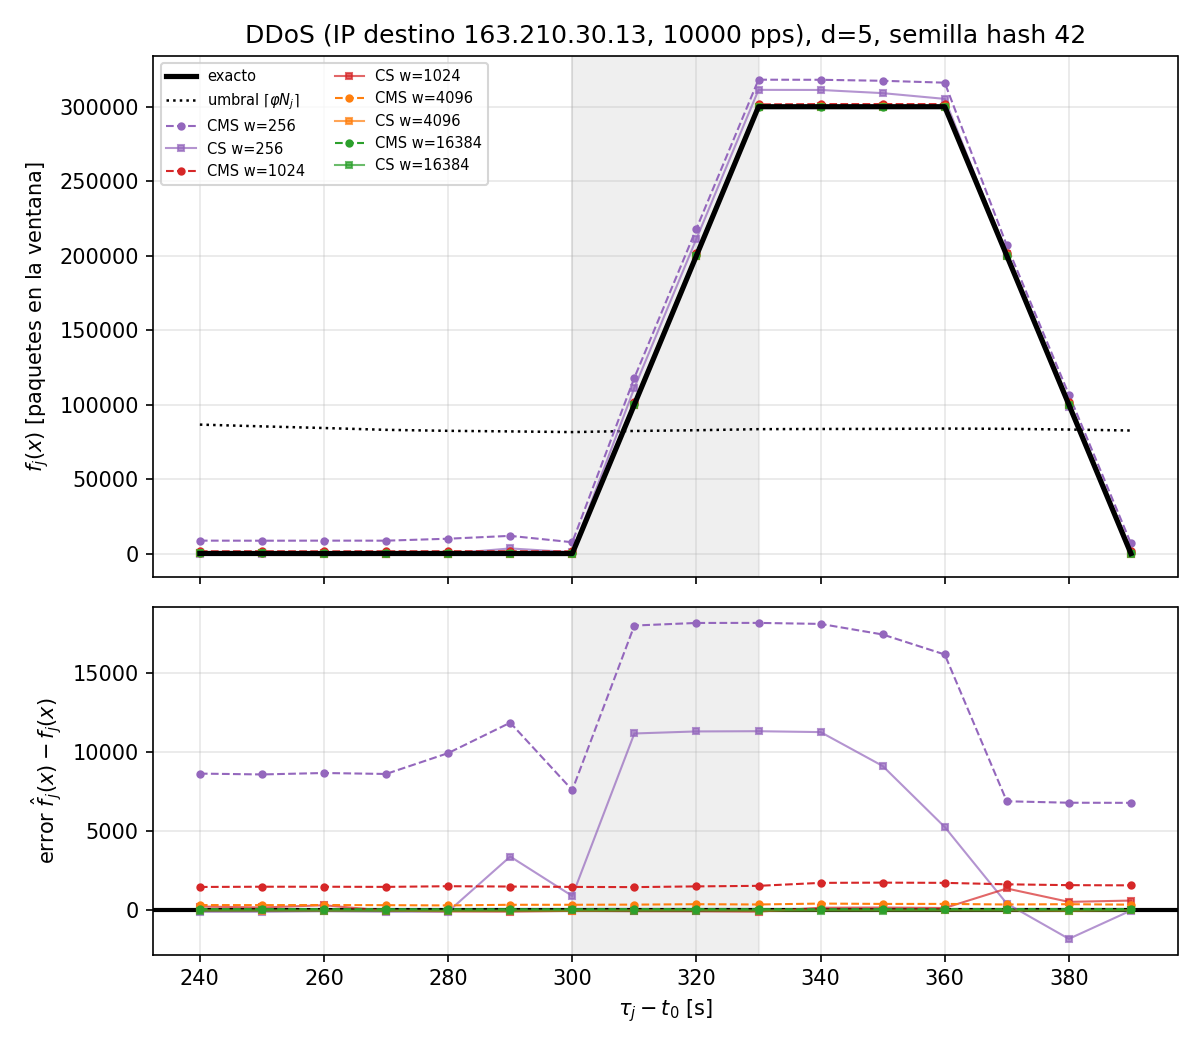
\includegraphics[width=\linewidth]{fig_ddos.png}\caption{DDoS (clave: IP destino).}\end{subfigure}\hfill
\begin{subfigure}{0.49\textwidth}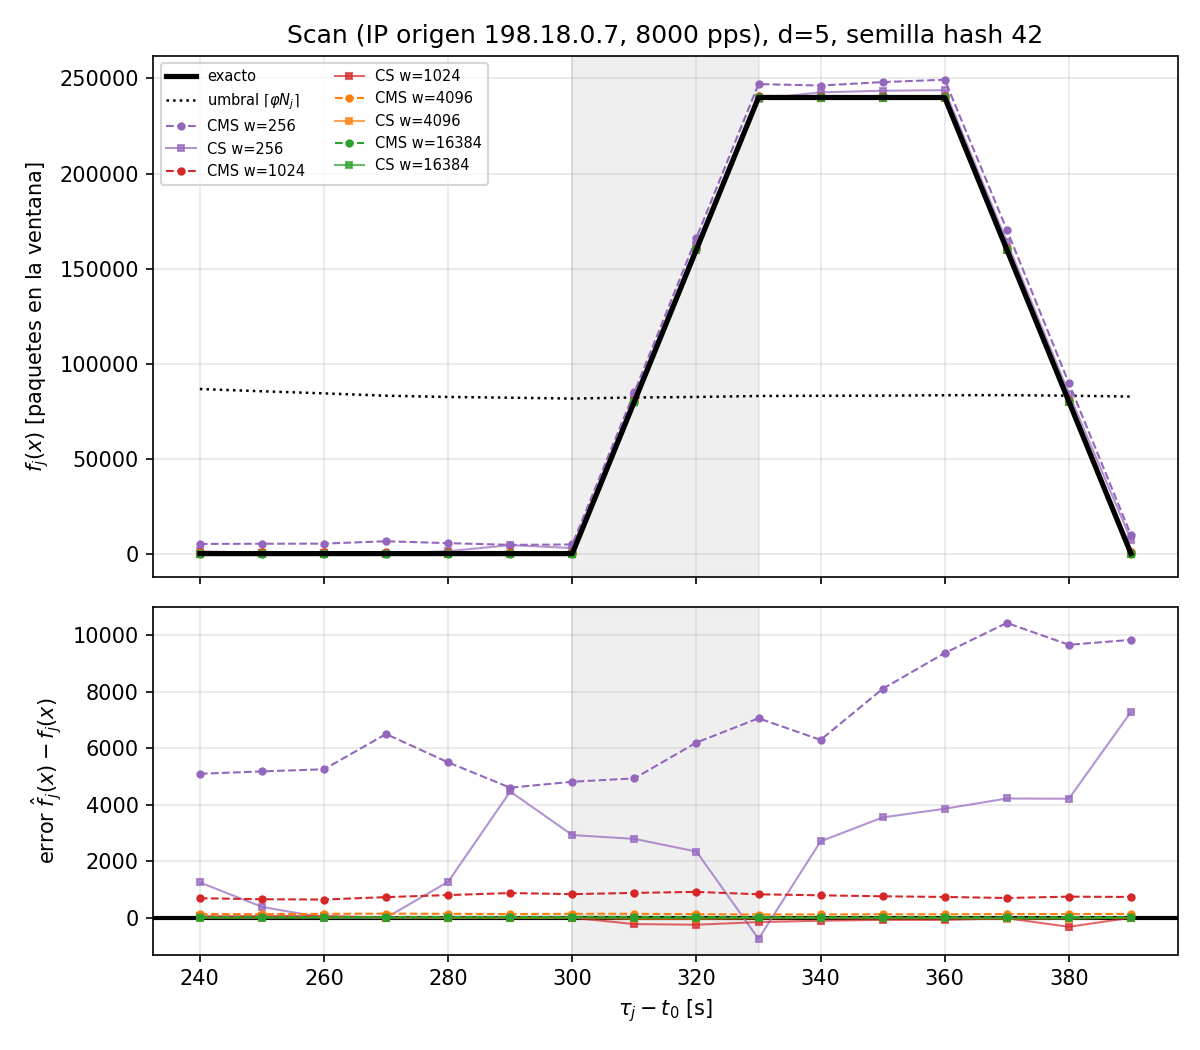
\includegraphics[width=\linewidth]{fig_scan.png}\caption{Scan (clave: IP origen).}\end{subfigure}
\caption{Frecuencia exacta y estimada entre 240 y 390\,s (CMS y CS, cuatro anchos) y umbral $\lceil\varphi N_j\rceil$. Abajo, el error $\hat f_j-f_j$.}
\label{fig:frecuencia}
\end{figure}

\paragraph{Precisión y memoria.} Con la misma memoria, CS es entre 2 y 30 veces más preciso que CMS, y el MRE de CMS cae aproximadamente como $1/w$. El error de CMS es siempre positivo; el de CS tiene ambos signos y varía más entre semillas (con $w=256$ en el DDoS, media 0,016 y desviación 0,020), por lo que su MRE no es necesariamente monótono en $w$.

\paragraph{Latencia y falsos positivos.} En el DDoS, todas las configuraciones detectan a los 310\,s, igual que la referencia exacta: en 10\,s el ataque aporta 100\,000 paquetes frente a un umbral de $\approx$82\,000. En el scan, a los 310\,s el atacante lleva 80\,000 paquetes, justo bajo el umbral, y la referencia exacta detecta a los 320\,s. Con $w=256$, las $\approx$5\,000 colisiones que suma CMS (estima 84\,933 contra un umbral de 82\,149) le hacen declarar el ataque una ventana antes, y lo mismo ocurre a los 380\,s. Es el falso positivo esperado de un estimador que sobreestima, y ocurre con las tres semillas. CS también cruza con la semilla 42 por su ruido, pero con las semillas 7 y 1234 detecta junto con la referencia exacta. Desde $w=1024$ todas las decisiones coinciden con la referencia. Con ataques de 3\,000 paquetes/s (anexo) el MRE se triplica y la detección sigue coincidiendo con la exacta.

\section{Cambio de frecuencia $\Delta f_j(x)$}

\begin{figure}[H]
\centering
\begin{subfigure}{0.49\textwidth}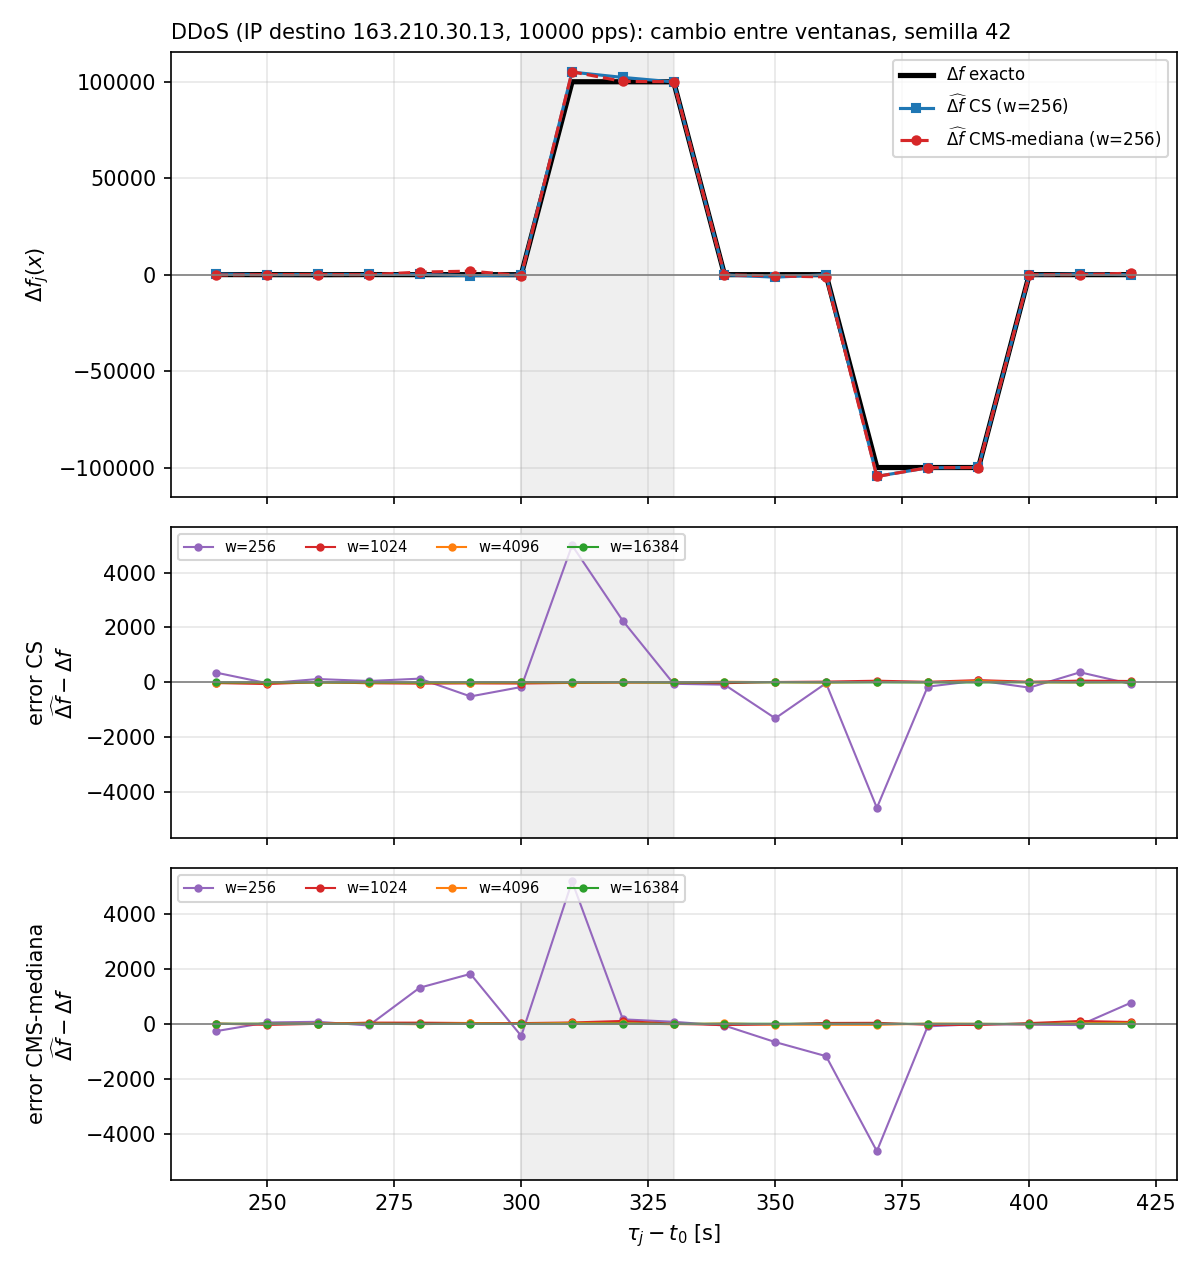
\includegraphics[width=\linewidth]{fig_delta_ddos.png}\caption{DDoS.}\end{subfigure}\hfill
\begin{subfigure}{0.49\textwidth}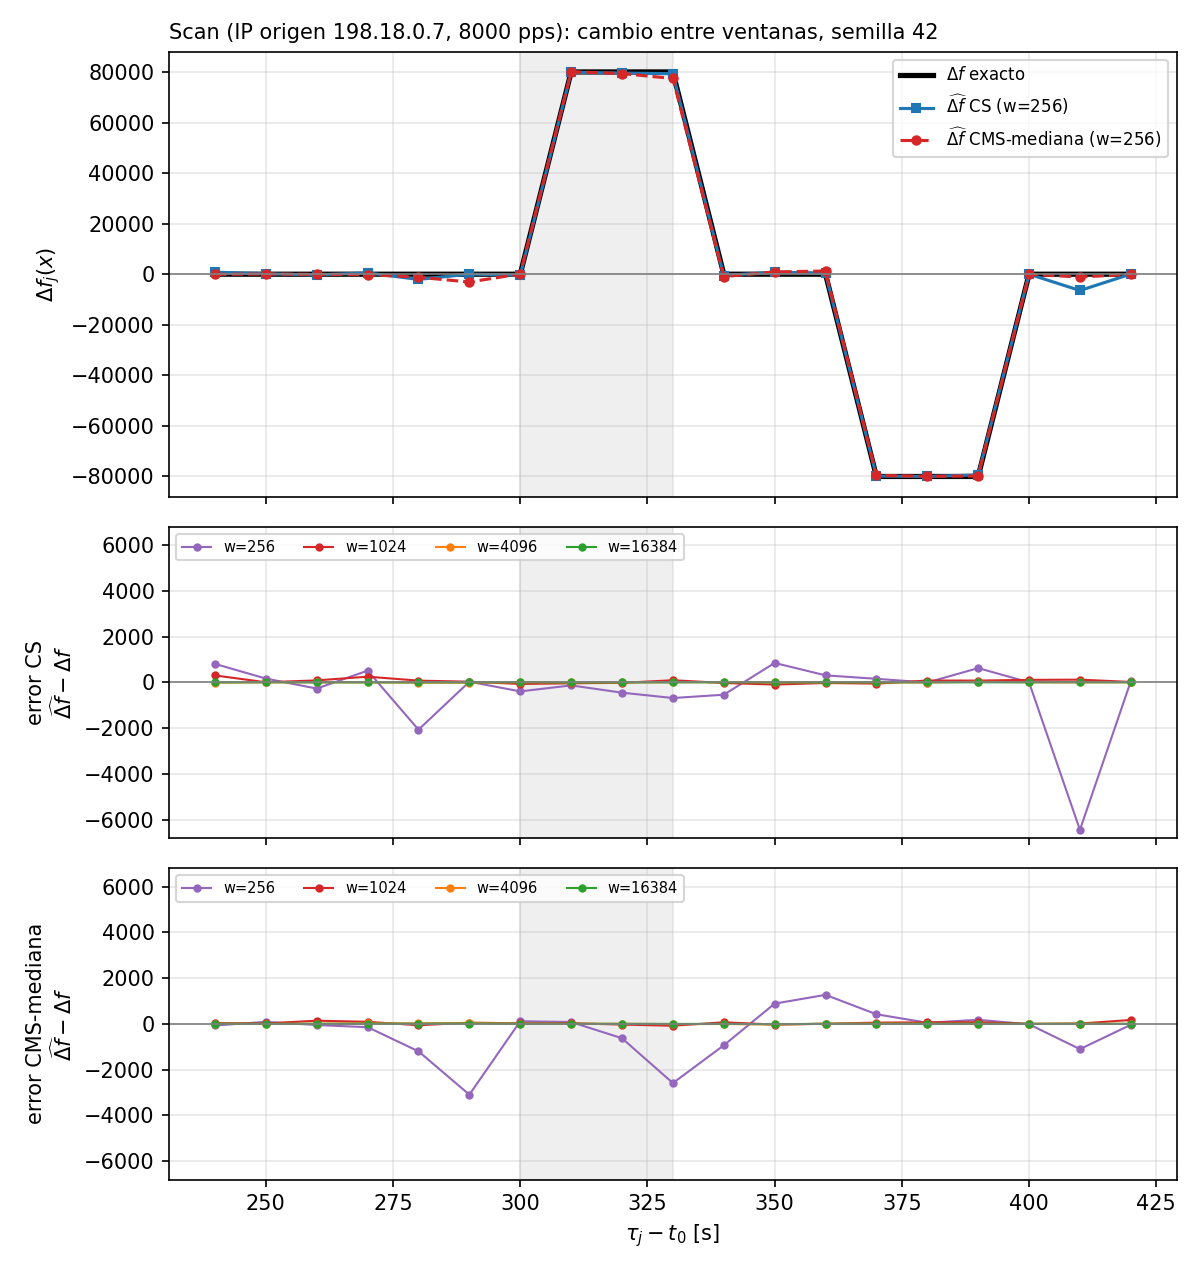
\includegraphics[width=\linewidth]{fig_delta_scan.png}\caption{Scan.}\end{subfigure}
\caption{$\Delta f_j$ exacto frente a CS y CMS-mediana ($w=256$); abajo, el error de cada estimador para los cuatro anchos.}
\label{fig:delta}
\end{figure}

El mayor incremento exacto ocurre a los 310\,s ($+100\,008$ en el DDoS, $+80\,000$ en el scan) y el mayor decremento a los 370\,s, cuando el ataque empieza a salir de la ventana ($-100\,007$ y $-80\,000$). Con $w=256$ no hay un ganador claro (Tabla~\ref{tab:delta} del anexo): en el DDoS, CS se equivoca algo menos en ambos extremos (4\,996 contra 5\,190 en el incremento); en el scan, CMS-mediana es mejor en el incremento (78 contra 133) y peor en el decremento (417 contra 155). Con $w=16384$ ambos aciertan con a lo más 3 paquetes de error. La diferencia está en las garantías: CS sigue siendo insesgado sobre un vector firmado y CMS-mediana no tiene cota conocida.

\section{Respuestas a las preguntas}

\begin{enumerate}[leftmargin=*]
\item \textbf{Linealidad.} El sketch de una unión de flujos es la suma de sus sketches, así que el de la ventana es la suma de los de sus subventanas. Al avanzar basta restar el que sale y sumar el que entra: $2dw$ contadores, sin recorrer los paquetes de la ventana.

\item \textbf{Error al reducir $w$.} Ambos crecen por colisiones, aproximadamente como $1/w$. En CMS todas las colisiones suman: el error es positivo y similar para todas las claves, y el mínimo sólo lo acota. En CS los signos aleatorios cancelan las colisiones en promedio y la mediana descarta las filas peores, así que el error es menor pero tiene ambos signos y fluctúa entre semillas.

\item \textbf{Ataque más claro y claves.} El DDoS: supera el umbral con holgura en la primera ventana y todas las configuraciones coinciden con la referencia. El scan queda justo bajo el umbral al inicio, y ahí aparecen los falsos positivos. La clave cambia porque el DDoS concentra el tráfico en un destino (muchas fuentes, una víctima) y el scan en un origen (un atacante, muchos destinos).

\item \textbf{Qué aporta $\Delta f_j$.} $f_j$ integra 60\,s: sube y baja gradualmente y sigue alta hasta 60\,s después del ataque. $\Delta f_j$ marca el instante en que cambia la tasa, con un salto positivo al inicio (310\,s) y uno negativo cuando el ataque sale de la ventana (370\,s), sin depender del nivel de fondo.

\item \textbf{CS frente a CMS-mediana.} Cada fila de CS, $s_i(x)\,\Delta A_j[i][h_i(x)]$, es un estimador insesgado aunque el vector tenga valores negativos, porque las colisiones entran con signo aleatorio; la mediana conserva su cota habitual. El mínimo de CMS se justifica sólo si cada fila sobreestima, lo que exige frecuencias no negativas. En $\Delta A_j$ las colisiones tienen cualquier signo y no se cancelan, así que la mediana de CMS puede quedar sesgada y no tiene garantía, aunque en estos datos ambos estimadores fueron comparables.
\end{enumerate}

\section{Conclusiones}

La linealidad permite mantener la ventana con costo $O(dw)$ por rotación, y la autoverificación de $N_j$ asegura la alineación con la referencia exacta. Con la misma memoria, CS es más preciso y no tiene sesgo, aunque su error varía más entre semillas; CMS sobreestima, lo que con anchos pequeños adelanta la detección. Desde $w=1024$ (140\,KiB por sketch) ambos reproducen las decisiones exactas en los dos ataques.

\section{Referencias}

\begin{itemize}
    \item MAWI Working Group Traffic Archive, samplepoint-F, 2018-12-03 14:00. \url{https://mawi.wide.ad.jp/mawi/}
    \item G.~Cormode y S.~Muthukrishnan. \emph{An improved data stream summary: the count-min sketch and its applications}. Journal of Algorithms, 55(1):58--75, 2005.
    \item M.~Charikar, K.~Chen y M.~Farach-Colton. \emph{Finding frequent items in data streams}. ICALP 2002, LNCS 2380, pp.~693--703.
\end{itemize}

\newpage
\appendix
\section{Anexo}

\subsection{Validación sin ataque}

\begin{table}[H]
\centering\small
\caption{Error absoluto medio (EA) y relativo medio (ER) sin ataque, sobre todas las ventanas. Tablas completas en \code{resultados/validacion.md}.}
\label{tab:validacion}
\begin{tabular}{llrrrrr}
\toprule
Clave & Grupo & $w$ & EA CMS & ER CMS & EA CS & ER CS \\
\midrule
dst & alta & 256   & 7\,740 & 3,22   & 2\,020 & 0,846 \\
dst & alta & 1024  & 1\,540 & 0,702  & 234    & 0,0615 \\
dst & alta & 4096  & 352    & 0,157  & 60,1   & 0,0134 \\
dst & alta & 16384 & 78,7   & 0,0351 & 7,38   & 0,00282 \\
\addlinespace
dst & baja & 256   & 7\,700 & 1\,230 & 759    & 94,4 \\
dst & baja & 16384 & 79,1   & 12,4   & 5,86   & 0,773 \\
\addlinespace
src & alta & 256   & 5\,980 & 36,9   & 3\,590 & 11,5 \\
src & alta & 1024  & 765    & 4,97   & 415    & 0,481 \\
src & alta & 4096  & 125    & 0,809  & 50,5   & 0,214 \\
src & alta & 16384 & 21,5   & 0,164  & 5,40   & 0,0447 \\
\addlinespace
src & baja & 256   & 6\,290 & 1\,570 & 2\,230 & 399 \\
src & baja & 16384 & 19,9   & 4,95   & 3,36   & 0,735 \\
\bottomrule
\end{tabular}
\end{table}

\subsection{Extremos de $\Delta f$}

\begin{table}[H]
\centering\small
\caption{Error en los extremos de $\Delta f$ y error absoluto medio (MAE) sobre toda la traza (semilla 42).}
\label{tab:delta}
\begin{tabular}{llrrrrrr}
\toprule
 & & \multicolumn{2}{c}{Incremento (310\,s)} & \multicolumn{2}{c}{Decremento (370\,s)} & \multicolumn{2}{c}{MAE} \\
\cmidrule(lr){3-4}\cmidrule(lr){5-6}\cmidrule(lr){7-8}
Ataque & $w$ & CS & CMS-med & CS & CMS-med & CS & CMS-med \\
\midrule
DDoS & 256   & 4\,996 & 5\,190 & $-4\,576$ & $-4\,644$ & 345,9 & 379,5 \\
DDoS & 1024  & $-20$  & 48     & 60        & 36        & 64,7  & 70,1 \\
DDoS & 16384 & 1      & 1      & $-2$      & 0         & 2,35  & 2,64 \\
\addlinespace
Scan & 256   & $-133$ & 78     & 155       & 417       & 447,8 & 365,9 \\
Scan & 1024  & $-40$  & 25     & $-55$     & 52        & 58,0  & 52,0 \\
Scan & 16384 & $-3$   & 0      & $-1$      & $-1$      & 1,92  & 2,58 \\
\bottomrule
\end{tabular}
\end{table}

\subsection{Ataques de baja intensidad}

Para que el error de los sketches se note más (§2 del enunciado), se repitieron ambos ataques con 3\,000 paquetes/s. El MRE con $w=256$ sube a 0,252 (CMS) y 0,130 (CS) en el DDoS, y a 0,138 y 0,058 en el scan. Todas las configuraciones detectan a los 30\,s, igual que la referencia exacta, sin falsos positivos. Las figuras están en \code{resultados/fig\_*\_bajo.png}.

\subsection{Reproducibilidad}

\code{codigo\_entregado/run\_experimentos.sh} compila, prepara las trazas, corre \code{exact\_hh} y \code{sliding\_sketch} y genera las figuras y tablas en \code{codigo\_entregado/resultados/}; las instrucciones están en el \code{README.md}. Los ataques usan la semilla 42 y los hashes las semillas 42, 7 y 1234.

\end{document}
